\documentclass[english]{article}\usepackage[]{graphicx}\usepackage[]{color}
%% maxwidth is the original width if it is less than linewidth
%% otherwise use linewidth (to make sure the graphics do not exceed the margin)
\makeatletter
\def\maxwidth{ %
  \ifdim\Gin@nat@width>\linewidth
    \linewidth
  \else
    \Gin@nat@width
  \fi
}
\makeatother

\definecolor{fgcolor}{rgb}{0.345, 0.345, 0.345}
\newcommand{\hlnum}[1]{\textcolor[rgb]{0.686,0.059,0.569}{#1}}%
\newcommand{\hlstr}[1]{\textcolor[rgb]{0.192,0.494,0.8}{#1}}%
\newcommand{\hlcom}[1]{\textcolor[rgb]{0.678,0.584,0.686}{\textit{#1}}}%
\newcommand{\hlopt}[1]{\textcolor[rgb]{0,0,0}{#1}}%
\newcommand{\hlstd}[1]{\textcolor[rgb]{0.345,0.345,0.345}{#1}}%
\newcommand{\hlkwa}[1]{\textcolor[rgb]{0.161,0.373,0.58}{\textbf{#1}}}%
\newcommand{\hlkwb}[1]{\textcolor[rgb]{0.69,0.353,0.396}{#1}}%
\newcommand{\hlkwc}[1]{\textcolor[rgb]{0.333,0.667,0.333}{#1}}%
\newcommand{\hlkwd}[1]{\textcolor[rgb]{0.737,0.353,0.396}{\textbf{#1}}}%

\usepackage{framed}
\makeatletter
\newenvironment{kframe}{%
 \def\at@end@of@kframe{}%
 \ifinner\ifhmode%
  \def\at@end@of@kframe{\end{minipage}}%
  \begin{minipage}{\columnwidth}%
 \fi\fi%
 \def\FrameCommand##1{\hskip\@totalleftmargin \hskip-\fboxsep
 \colorbox{shadecolor}{##1}\hskip-\fboxsep
     % There is no \\@totalrightmargin, so:
     \hskip-\linewidth \hskip-\@totalleftmargin \hskip\columnwidth}%
 \MakeFramed {\advance\hsize-\width
   \@totalleftmargin\z@ \linewidth\hsize
   \@setminipage}}%
 {\par\unskip\endMakeFramed%
 \at@end@of@kframe}
\makeatother

\definecolor{shadecolor}{rgb}{.97, .97, .97}
\definecolor{messagecolor}{rgb}{0, 0, 0}
\definecolor{warningcolor}{rgb}{1, 0, 1}
\definecolor{errorcolor}{rgb}{1, 0, 0}
\newenvironment{knitrout}{}{} % an empty environment to be redefined in TeX

\usepackage{alltt}
\usepackage{fancyhdr}
\pagestyle{fancy}
\setlength{\parskip}{\smallskipamount}
\setlength{\parindent}{0pt}
\usepackage{amsthm}
\usepackage{amsmath}
\usepackage{wrapfig}
\usepackage{graphicx}
\graphicspath{{../figures/}}
\usepackage{float}
\usepackage[margin=0.5in]{geometry}

\IfFileExists{upquote.sty}{\usepackage{upquote}}{}
\begin{document}


\title{Lab 1 - Redwood Data\\
Stat 215A, Fall 2014}

\author{Xiang (Lisha) Li}

\maketitle

\section{Introduction}

The Redwoods dataset was collected to get a high resolution idea of the microclimate around a redwood tree over time. The project was motivated by recent developments in measurement equipment, in particular in wireless motes, that allowed for a large amount of detailed data to be collected. 

\section{The Data}
Data from two redwood trees (interior and exterior) was collected over 44 days in early summer, when the most dynamic microclimatic variation was expected. Recordings were taken by 33 one inch motes every 5 minutes starting from a height of 15 meters to 70 meters on both tree, captured mostly on the west side, and spaced 0.1-1 meters from the trunk.  These heights were chosen to concentrate on the foliage region, so climate measurements are more buffered against environmental effects, and thus were expected to be more an indication of the microclimate influence by the tree.  \\

Each mote had 4 sensors, one for temperature, humidity, ambient and direct photosynthetically active solar radiation (hamatop and hamabot respectively). The design of the mote seemed reasonably thought out to measure these quantities properly.  For instance the ambient PAR sensor was sheltered but had wide reach, and mote sensors were calibrated to ensure measurements between motes agreed within reasonable levels.

\subsection{Data Collection }

The data was collected via wireless download every 5 minutes, comprising the net dataset, and was recorded locally on a 512 kB chip (enough for the duration of the measurements, unless the chip was partially full from testing), comprising the log dataset. This turned out to be useful redundancy, since during the data cleaning, one can check that the intersection of their recorded values was 60\% of the net data and only 20\% (approx.) of log data.

\subsection{Data Cleaning}

The data cleaning is best summarized in two parts. I first systematically checked the hamatop, hamabot, temperature, humidity and voltage measurements of both net and log datasets for abnormalities, plotting against epoch as a guide. In the second part, I combined net, log and locs data, and verified the all dataset had no extra information. Details and code are documented in the Lab1dataclean file (with a outline of where to find each section by code line, and includes analysis of the Redwood paper's outlier rejection).  Details for Part I and II of the cleaning now follow.\\

{\bf Part I}
Aside from checking abnormalities in range and spread of the variable measurements, I assumed that temperature and humidity should evolve smoothly over time (epoch), and expected at least a noticeable pattern of day and night in the hamabot, hamatop measurements, so I was not alarmed that they climbed dramatically at periodic peaks.  Hamabot and hamatop displayed more erratic ups and downs during the day compared to temperature and humidity, this finding was consistent across all motes (later confirmed via plots in data exploration).  I was not concerned with the more dramatic fluctuations in hamatop/bot findings as it is plausible light distribution is more extreme than temperature and humidity. Especially since the measurements were in Kelvin colour units.  Through a quick google search, one finds that 5000K corresponds to a cloudy sky, 10 000 in hamatop readings corresponds to a clear blue sky, and a low of 1500 corresponds to light from a candle.  With this in mind, the fluctuations seen by hamabot/top was no cause for alarm (see figure 1 for an example from node135). Different light sources can easily be block by trivial changes such as wind blown leaves, hence the huge variation in hamatop/bot measurements within several epoch counts also passed my data cleaning.  In contrast I assumed a far greater number of forces need to be aligned to dramatically shift temperature and humidity recordings between several epochs, so I was vigilant about detecting erratic jumps in these variables per mote. \\
 
Staring with log and humidity, I noticed nodes 29, 198 and 65535 were responsible for negative humidity readings. I discovered 29 produced constant humidity and constant temperature readings for the entire duration of the study, so concluded it had a faulty humidity and temperature sensor.  The hamabot/top readings did not go past epoch 600, which was too small to even verify periodicity, though the readings were within reasonable range.  Thus I decided not to take a risk and deleted the (few and faulty) records of node 29. \\

198 simply had one outlier that produced a negative humidity reading (I checked the distributions by plotting all its other variable readings against time), so I deleted the one outlier (set to NA).  Finally node 65535 produced just measurements for one epoch, so I deleted the mote's data, nothing was within reasonable bounds (over 600 $^{\circ}C$ temperature, highest hamatop/bot readings).  \\

For log and temperature, everything was reasonably behaved (I already deleted the faulty node 29's temperature readings).  There were some subzero temperatures, dropping during the evening as cross referenced with hamatop epoch's, but that was not strong enough cause for deletion, though suspicious for a California spring.   \\

For hamabot/top in log, there was one outrageous outlier, while everything else stayed within bounds.  Investigating, the outlier was produced by nodeid 40, which basically went awry after some time for both hamatop and hamabot readings.  Recordings also did not last past epoch 100, so it was not a loss to delete both readings from the dataset.  \\

Lastly, for log, I looked at the voltage and the only strange thing I noticed was that nodes 128, 134, 135, 141, 142, 143, 145 had constant readings for the voltage (constant and close to zero). I investigated the other measurements taken by these nodes and plotted them against time, and found them all acceptable. I then dug into the network topology and checked neighbouring motes to see if the measurements were similar, and found no alarming difference, which confirmed my decision to keep their measurements, and only throw out their voltage recordings (set to NA).  \\

Just to be safe, I also looked at relationships pairwise between the variables and did not arrive at further justification for removal. Cleaning the net dataset encountered similar problems as for log, details can be found in the enclosed code.   \\

{\bf Part II}

\begin{wrapfigure}{r}{0.3\textwidth}
 \vspace{-40pt}
  \begin{center}
    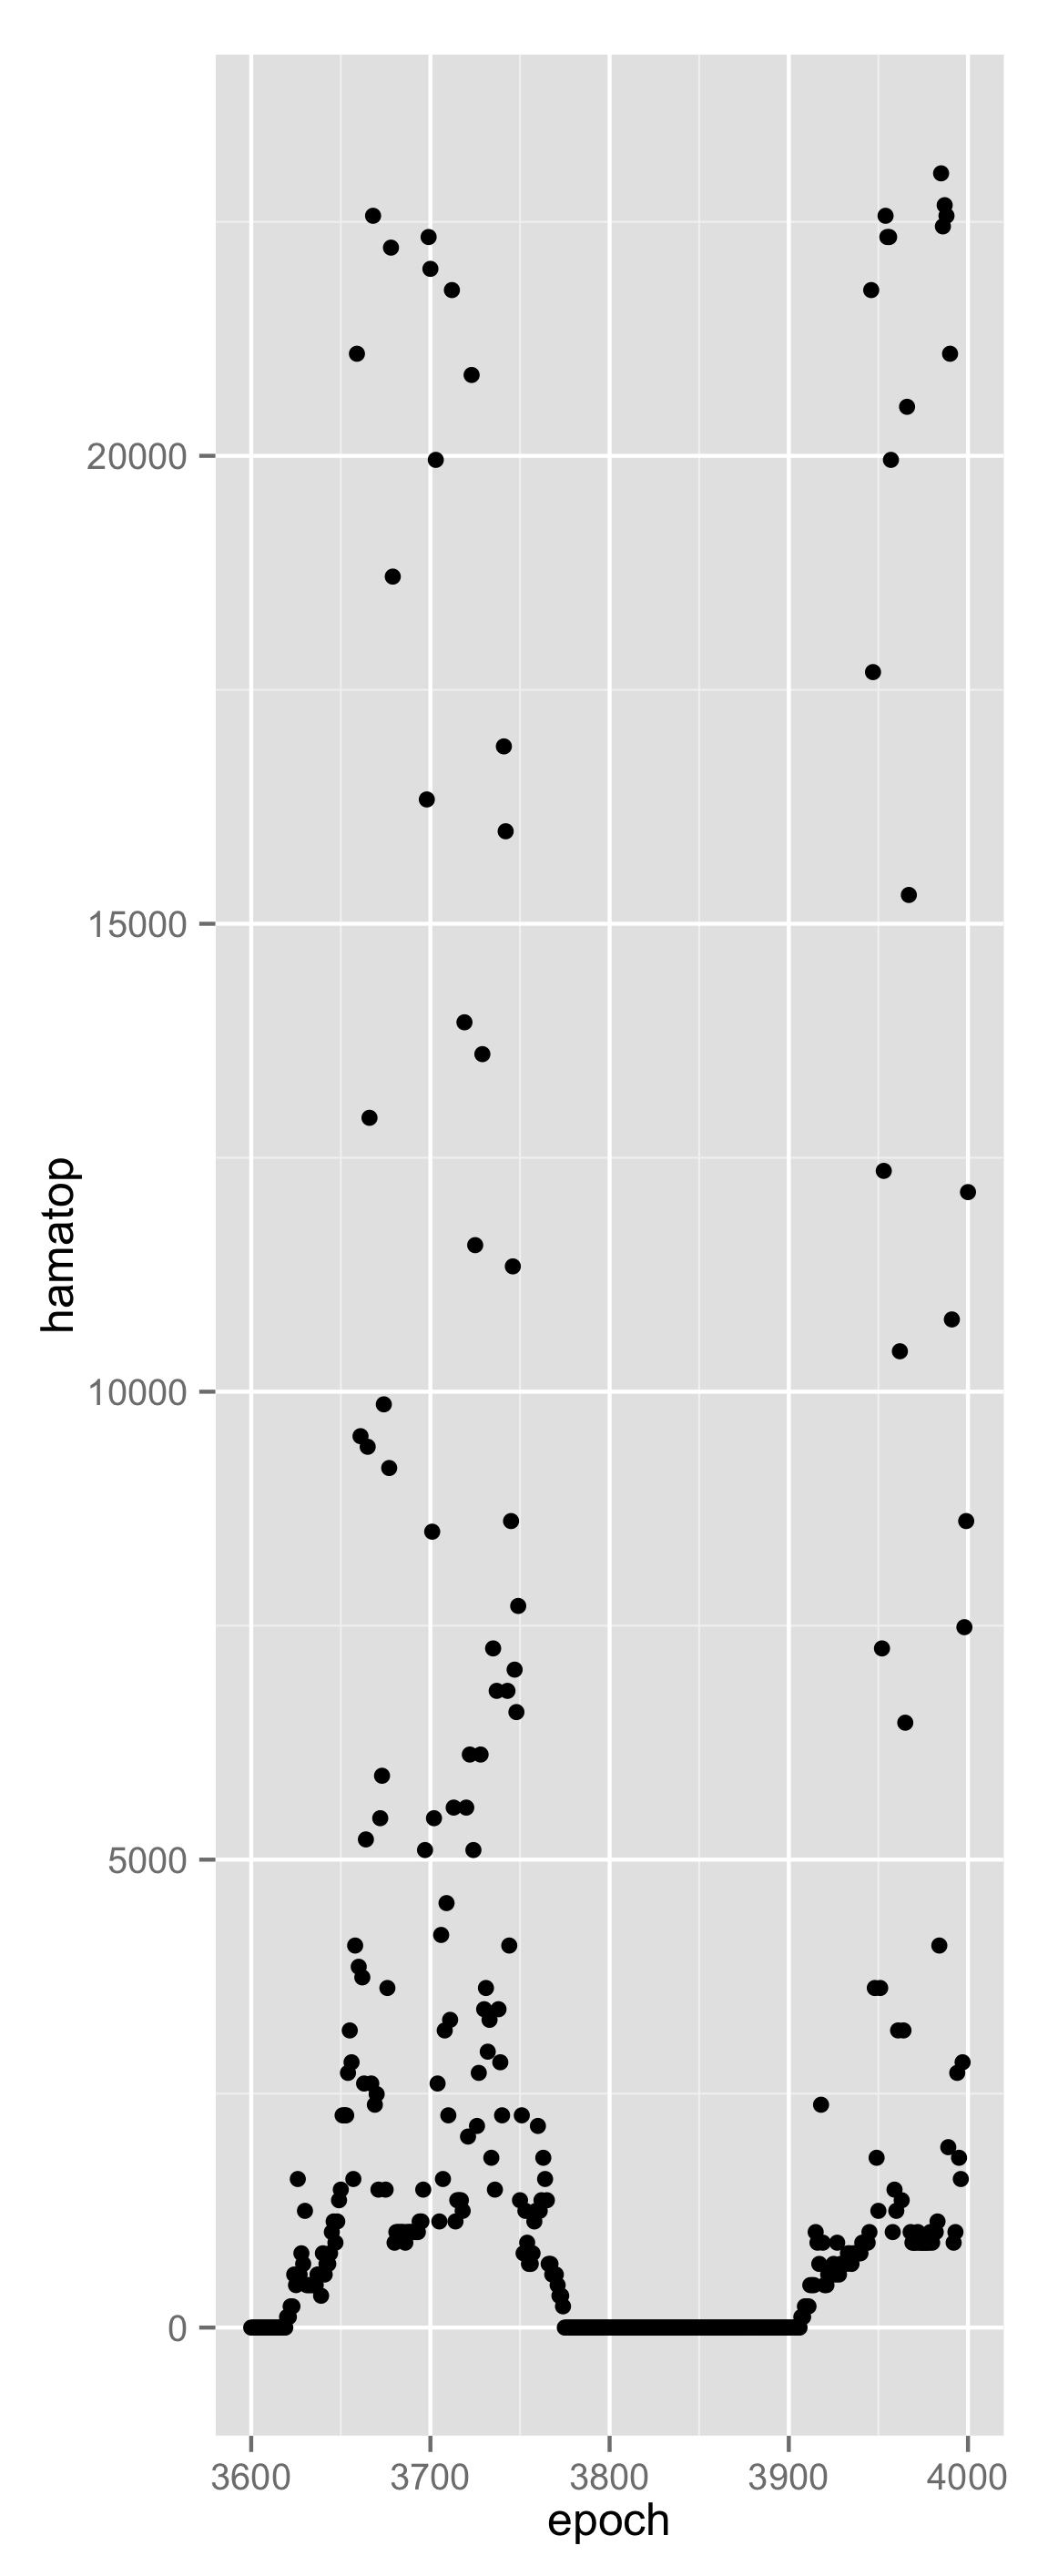
\includegraphics[scale=0.1]{node135example.png}
  \end{center}
   \vspace{-20pt}
  \caption{node135}
\end{wrapfigure}

Before combining the three datasets, I removed multiple entries (starting at line 500 of Lab1data.clean code).  For both log and net, I checked for differences in records of repeated entries (each nodeid-epoch pair should have the same observation) and inspected the nodeid-epoch pairs for which a reading in voltage, hamatop, hamabot, temperature or humidity differed.  The multiple entries had mostly the same number of records, and when they did differ, the spread of this difference was negligible so I just replaced the values with the average of the two. I defined `negligible' by first defining a normalized difference measurement as (min(variable)-min(variable))/max(variable) and then checking the spread of this count.  The normalized difference will be less than or equal to 1, and gives me a sense of the difference in measurements relative to the value of the measurement. For example, the log.doubles dataset (double entries from log) gave me 10 node-epoch pairs on which the temperature measurement differed.  But a summary of the spread of this normalized difference shows that taking the mean of both entries did not alter measurements by much:
Min.   :0.000e+00        
1st Qu.:0.000e+00        
Median :0.000e+00        
Mean   :4.786e-05        
3rd Qu.:0.000e+00        
Max.   :4.974e-02   
\\
For the few variables where the difference between repeated entries was large, I individually looked at what was going on in the times close to the differing incident (i.e went back to net or log and graphed the variables around the epoch times where the disagreement happened).  These large differences exclusively came from hamatop and hamabot readings. For instance, in the case of node135 (figure.1), I realized that the readings were coming from a particularly erratic time of light change, so decided to average the values despite the large range ($\sim$500 versus $\sim$2000). Choosing between 500K and 2000K qualitatively is like choosing between whether the mote witnessed candle-like intensity of light, or barely any light. Thus averaging did not seem less interpretable then taking max or min (that is, we can interpolate an experience between the two qualia).
\begin{wrapfigure}{r}{0.4\textwidth}
\vspace{-30pt}
  \begin{center}
    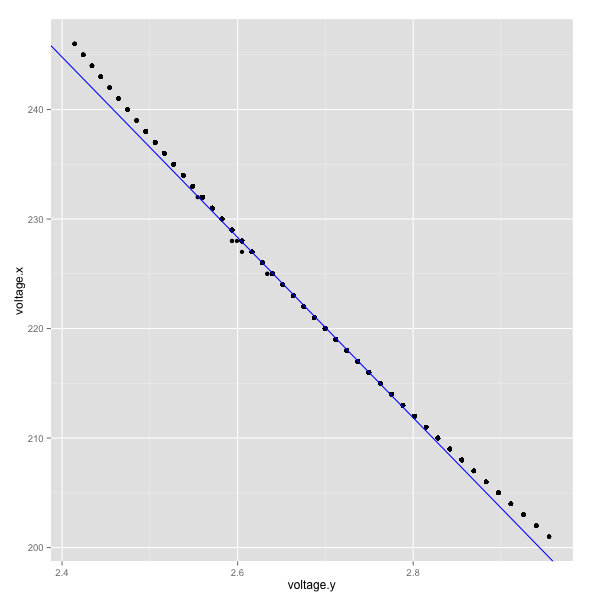
\includegraphics[height = 200pt]{voltagecalibration.png}
  \end{center}
  \vspace{-20pt}
  \caption{Voltage Calibration}
     \vspace{-20pt}
\end{wrapfigure}

After duplicates were removed from net and log, I finally did an inner join to investigate the observations on which the two intersected. I first looked at whether the recordings at their intersection matched. They generally agreed. On the recordings that they disagreed, the spread of their normalized difference was too small to be significant (same analysis done when dealing with multiples in log/net individually), so I replaced both values with their mean. I also calibrated the conversion between the voltage measured by net and log by running a linear regression (figure.2) and used the regression line to convert to the voltage units used in the log dataset.  This allowed me to address their outlier rejection method in the following section. Finally, I left joined the combined net-log data with the locs data in order to associate the spatial information of each mote in a final combined dataset. Only a few nodes of my net-log dataset was not covered by locs data.  

\subsection{Outlier rejection}
The Redwoods paper's outlier rejection was problematic for several reasons. A priori, I worried that voltage may be correlated with subsets of the variables. For instance, it may be the case that higher humidity caused the voltage to drop below 2.4. If we throw away all readings from nodes whose voltage drops below 2.4, we end up biasing our data against high humidity readings.  Below are scatterplots of the voltage readings with each of the four variables (voltage is on the x axis, redline at 2.4 volts). The plots use my cleaned dataset from the last section. The plots below also help demonstrate that the cleaned data already filtered out the outliers which prompted the Redwoods paper to reject readings from nodeid-epoch pairs with voltage below 2.4. The plots also confirm that voltage below 2.4 was valuable data. There are loose correlations between voltage and temperature, and voltage and humidity.  This supports my suspicion that deleting all observations from voltages below 2.4 was biasing our dataset. Observe also that low voltage correlated with the lowest hamatop/bot readings.  By throwing away observations taken at lower voltages, we bias the data against readings of extreme climatic conditions.  


\begin{figure}[H]
\centering
\begin{minipage}{.50\textwidth}
\centering
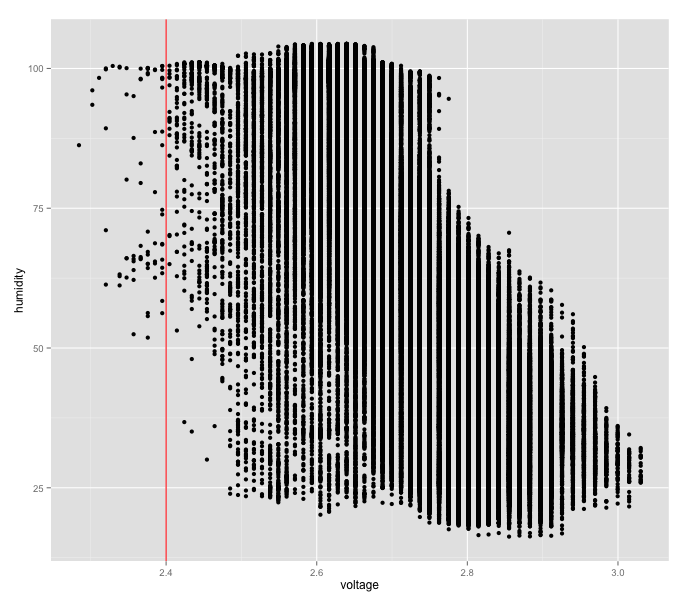
\includegraphics[width=180pt]{volthumid}
\vspace{-15pt}
\caption{Humidity}
\vspace{-10pt}
\end{minipage}\hfill
\begin{minipage}{.50\textwidth}
\centering
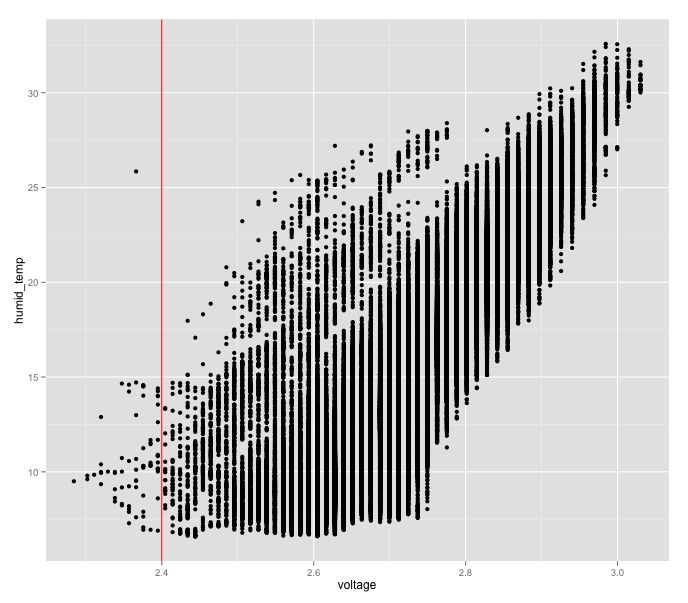
\includegraphics[width=180pt]{volttemp}
\vspace{-15pt}
\caption{Temperature}
\vspace{-10pt}
\end{minipage}\hfill
\end{figure}


\begin{figure}[H]
\centering
\begin{minipage}{.50\textwidth}
\centering
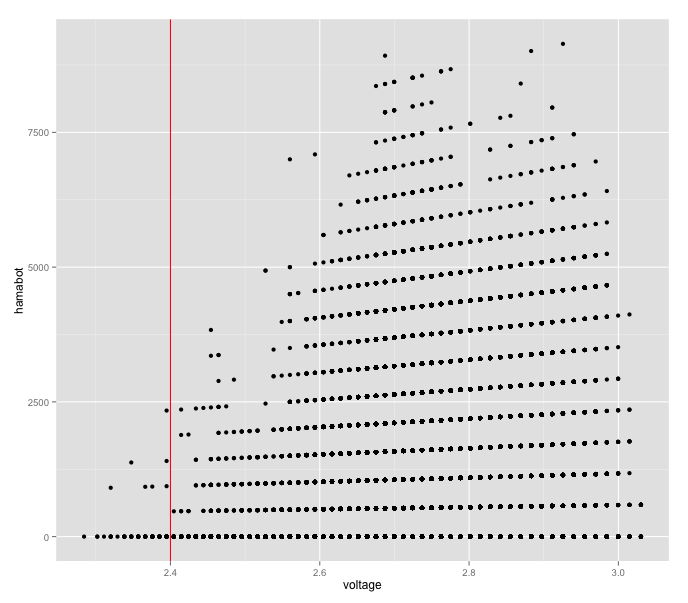
\includegraphics[width=180pt]{voltbot}
\vspace{-15pt}
\caption{Hamabot}
\vspace{-10pt}
\end{minipage}\hfill
\begin{minipage}{.50\textwidth}
\centering
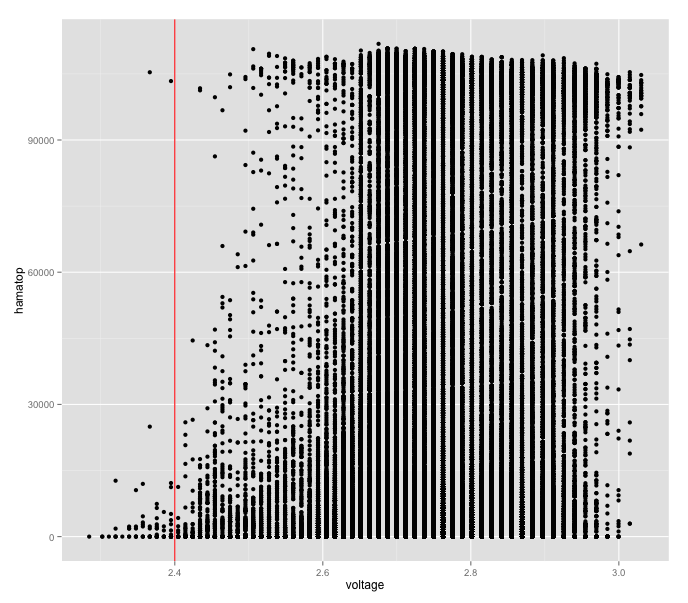
\includegraphics[width=180pt]{volttop}
\vspace{-15pt}
\caption{Hamatop}
\vspace{-10pt}
\end{minipage}\hfill

\end{figure}

\subsection{Data Exploration}

\begin{figure}[H]
\centering
\begin{minipage}{.70\textwidth}
\centering
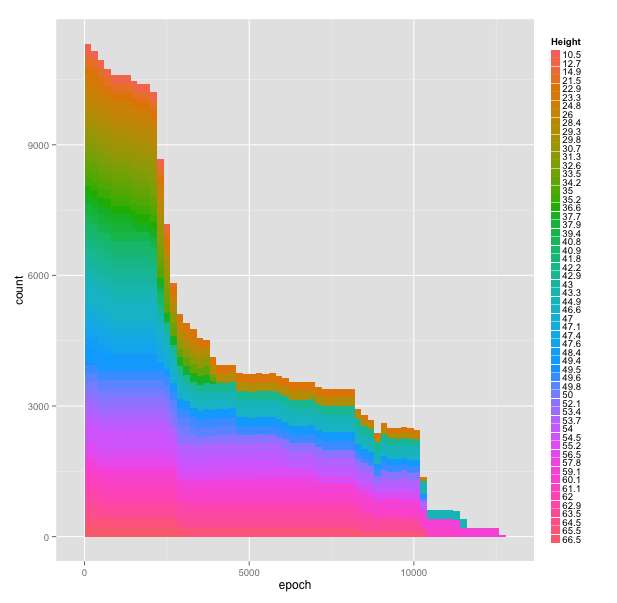
\includegraphics[width=\linewidth]{plot1}
\caption{Histogram of observation count in Epoch}
\label{fig:test1}
\end{minipage}\hfill
\begin{minipage}{.30\textwidth}
\centering
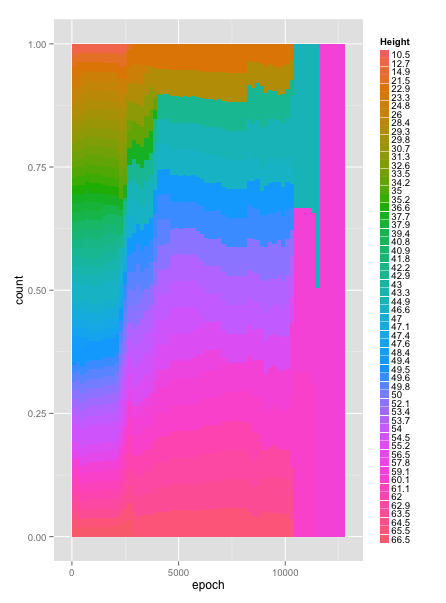
\includegraphics[width = \linewidth, height=300pt]{plot2}
\caption{Normalized Histogram}
\label{fig:test2}
\end{minipage}
\end{figure}

The first plot is a histogram of how many observations were taken in finely binned epoch intervals.  It is coloured by height to draw our attention to the distribution of heights at which the observations were taken.  The second graph is the normalized histogram to get a sense of what proportion of the observations came from each height.  This plot shows that that the number of measurements taken experienced roughly two phase transitions (I played around with different binning and this qualitative claim remained robust).  At around epoch 3000 we lose about half the observations, and at about epoch 8000 we loose approximately three quarters of the remaining observations. The height distribution also changes significantly at these phase transitions, as better illustrated by figure 8.  This was useful information to keep in mind when I explored other variables and was interested in how height affected their measurements varying with time. For instance,  if we noticed the average temperature increase dramatically at one of the aforementioned epoch transitions, we should keep in mind that the distribution of mote heights might have confounded this conclusion.  The distribution of where the motes were placed on on the tree was less variable in time, as most of the motes were placed on one side, so we did not show plots colouring by the direction information as it reveals less interesting things compared to considering height information.  \\    

Plots 9 and 10 are averaged timeseries of all the nodes, measuring temperature and humidity.  I once again coloured by height to bring out spatial correlations with this temporal data.  The colouring did not suggest that lower regions of the tree experienced more extreme variations in both variables, but I kept in mind that there were far less readings from motes at lower regions of the tree, and did not scale the colouring appropriately here.  Plot 11 and 12 study the same data as figure 10, but break it down to two epoch intervals to create two graphs.  In the first we notice far more dark points, which corresponds to measurements from motes in the lower regions of the tree.  This is because there were still many motes working at such height during epoch 0-2000.  Thus, figure 11, gives evidence to the hypothesis that lower regions of the tree experienced more extreme humidity better than figure 12 does.  The epoch interval figure 12's observations come from   is dominated by motes higher up in the trees, so we see less the contribution from lower motes.    
\begin{figure}[H]
\centering
\begin{minipage}{.50\textwidth}
\centering
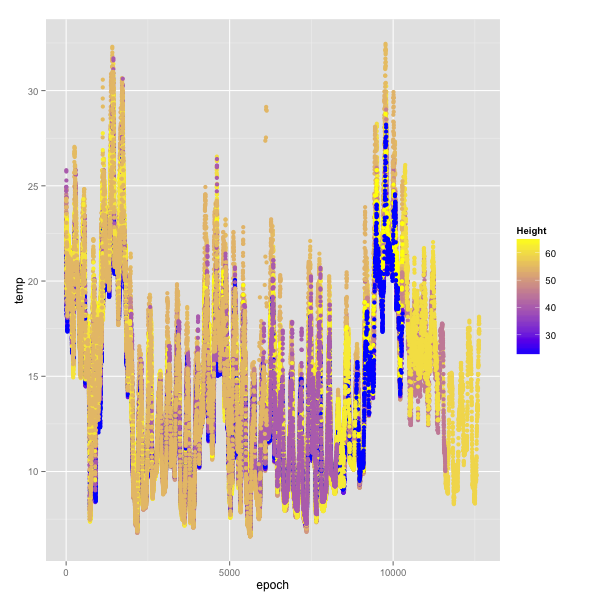
\includegraphics[width=\linewidth]{tempheight.png}
\caption{(Temperature, epoch, height}
\vspace{-10pt}
\end{minipage}\hfill
\begin{minipage}{.50\textwidth}
\centering
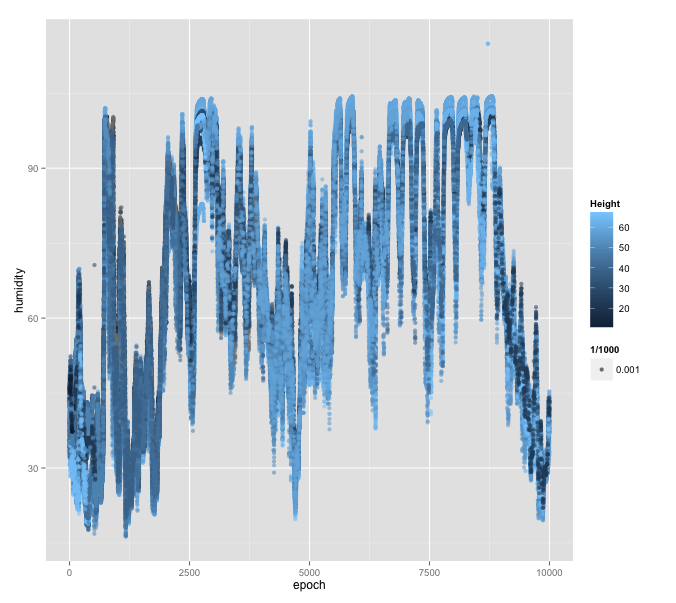
\includegraphics[width=\linewidth]{humidepoch}
\caption{(humidity, epoch, height)}
\vspace{-10pt}
\end{minipage}
\end{figure}



\begin{figure}[H]
\centering
\begin{minipage}{.50\textwidth}
\centering
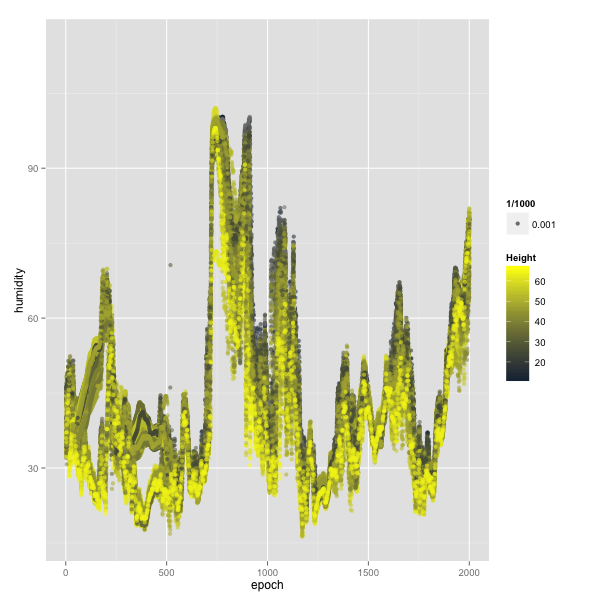
\includegraphics[width=\linewidth]{hum2}
\caption{(humidity, epoch (0-2000), height}
\vspace{-10pt}
\end{minipage}\hfill
\begin{minipage}{.50\textwidth}
\centering
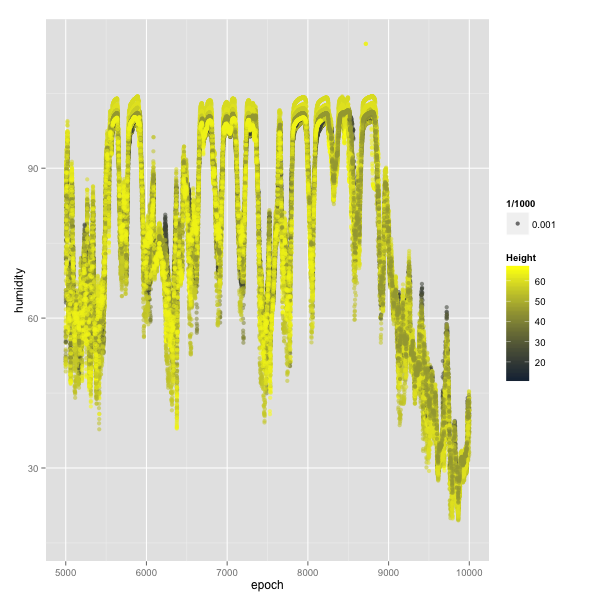
\includegraphics[width=\linewidth]{hum1}
\caption{(humidity, epoch (5000-10000), height)}
\vspace{-10pt}
\end{minipage}
\end{figure}


Plot 13 below shows that the concentration of eastward facing motes renders directional information hard to use when assessing how they are related to variable readings (too little data points with different directions).  Plot 14 shows us interesting hamatop variation in time, and colouring by height suggests that height does correlate with how much light these motes receive--hardly shocking, but pleasing to see in plot form with a light-like colour choice.   

\begin{figure}[H]
\centering
\begin{minipage}{.50\textwidth}
\centering
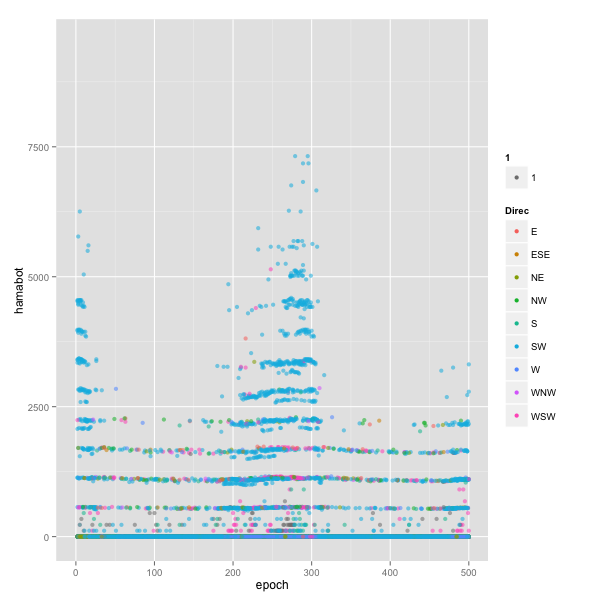
\includegraphics[width=\linewidth]{hamabotdirec}
\caption{(hamatop, epoch, height)}
\end{minipage}\hfill
\begin{minipage}{.50\textwidth}
\centering
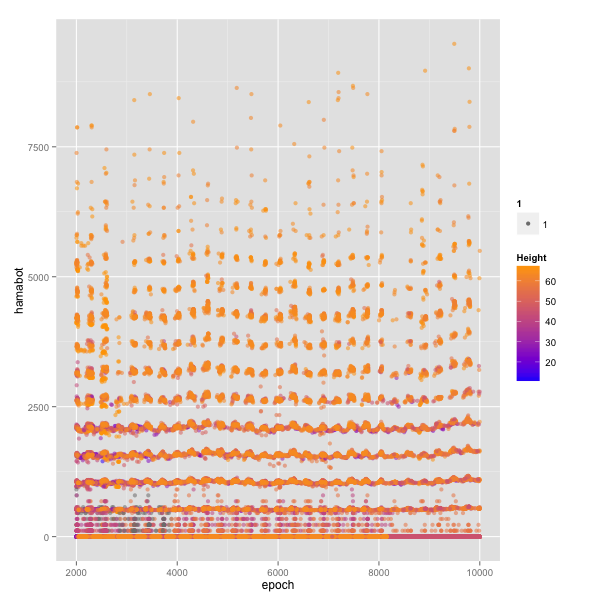
\includegraphics[width=\linewidth]{hamaheight}
\caption{(hama, epoch, height)}
\end{minipage}
\end{figure}

Node 42 had the most number of observations, so I studied various plots of its variables to get a sense of temporal variations of the variables.   
\begin{figure}[H]
\centering
\begin{minipage}{.50\textwidth}
\centering
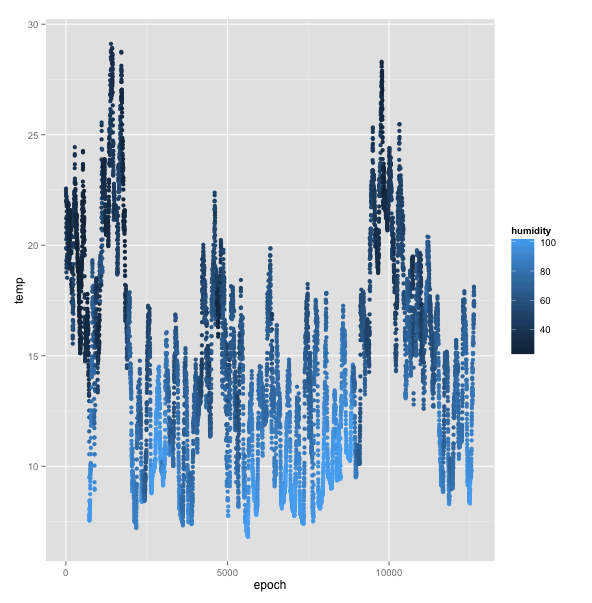
\includegraphics[width=\linewidth]{42epochtemphumid}
\caption{(Node 42: Temp vers Epoch (with Humid))}
\label{fig:test1}
\end{minipage}\hfill
\begin{minipage}{.50\textwidth}
\centering
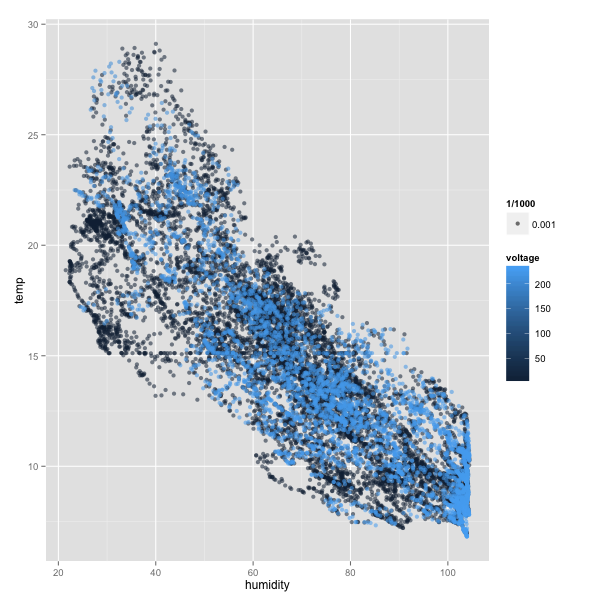
\includegraphics[width=\linewidth]{42temphumid}
\caption{(Node 42: Temp versus Humidity (with Voltage))}
\label{fig:test2}
\end{minipage}
\end{figure}

The first plot is a time-series of how temperature varies with time, coloured by the humidity.  This allowed me to witness a correlation between humidity and temperature, which I decided to explore further with a scatterplot.   Just to get an idea of whether voltage was effected by the two readings, I coloured the second plot by voltage.  Voltage does not look tightly correlated with the two variables, but humidity and temperature certainly have a correlation.  Though the residuals are large, but they look uniformly distributed, so using a linear model is justified (did not include residual plot here as it is quite obvious by inspection).  This plot also made curious about how temperature and humidity are related across motes. One thought was that if the trees was creating microclimates in its sheltered foliage, then it may have different temperature humidity correlation depending on the height of the tree.  I explored this hypothesis by first looking at the following plots. 

\begin{figure}[H]
\centering
\begin{minipage}{.60\textwidth}
\centering
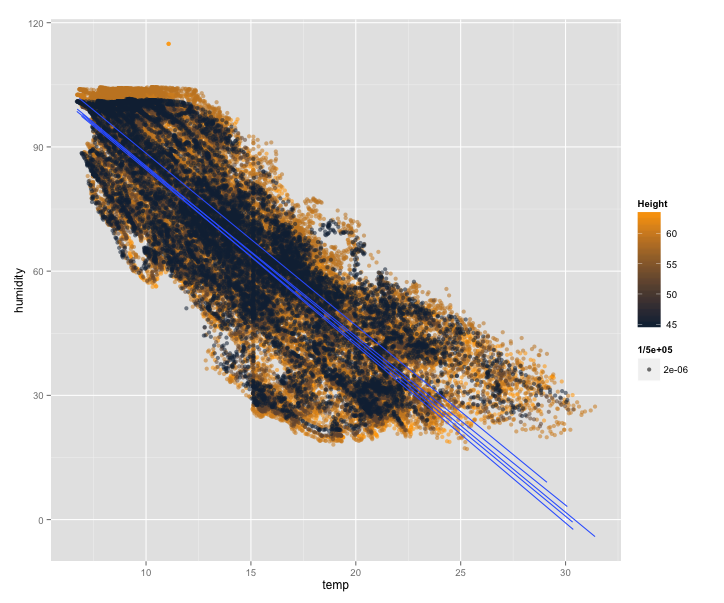
\includegraphics[width=\linewidth]{top5humidtemp}
\caption{(Humidity versus Temperature top 5 nodes}
\label{fig:test1}
\end{minipage}\hfill
\begin{minipage}{.40\textwidth}

In plot 17 we colour the points by height, and each line is a linear regression done to the nodes by their height group.  The plot gives strong evidence that humidity and temperature were correlated with the same slope across different heights. Initially I plotted the entire set of observations, but arrived at two outlier regression slopes.  I noticed they are from nodes that have very few observations, and hence they introduced a lot of noise.  Thus in plot 17, I only plotted data from the 5 nodes with the most observations.  

\end{minipage}
\end{figure}



But then I realized that these nodes included nothing below 40 meters (again lower region motes were underrepresented in observation), so I decided to randomly sample several nodes that have at least more than 7000 observations.  This was good enough to get a dense scatterplot, but allowed nodes from all heights to be included in the sample.  My faceted graph of this result is displayed in the findings section.   

I continued playing around with the data from the 5 nodes used in plot 17 to study correlations between height groupings and other variables.  The plots below concern the PAR variables, which unsurprisingly showed more variation in regression lines across height.    


\begin{figure}[H]
\centering
\begin{minipage}{.50\textwidth}
\centering
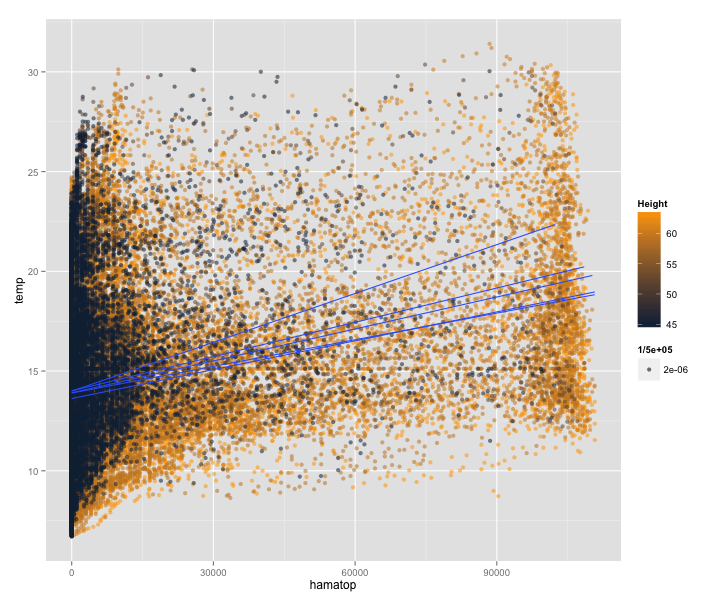
\includegraphics[width=\linewidth]{top5hama}
\caption{(hamabot, epoch, height}
\label{fig:test1}
\end{minipage}\hfill
\begin{minipage}{.50\textwidth}
\centering
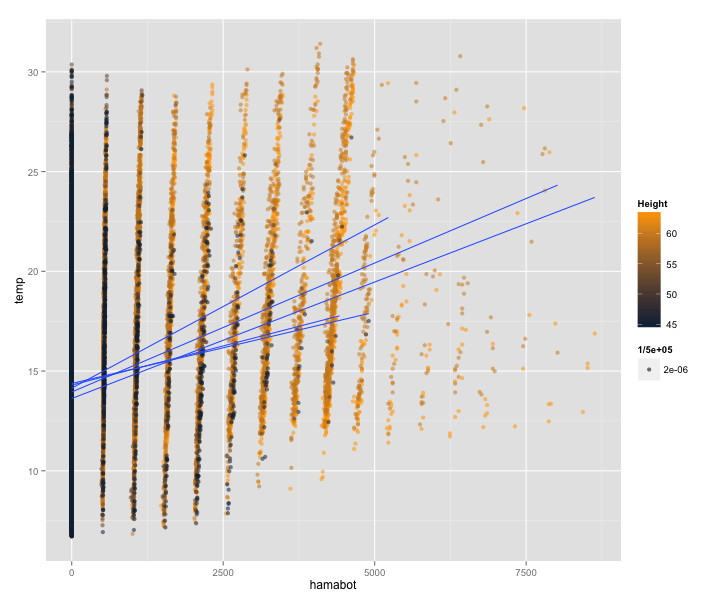
\includegraphics[width=\linewidth]{top5hama2}
\caption{(hamatop, epoch, height)}
\label{fig:test2}
\end{minipage}
\end{figure}

\section{Graphical Critique}

Let's begin with the plots in 3a. The plots do give some indication of the spread of the values, but not much else can be gleaned from them.  The data was collected to get a high resolution picture of how climate varies around a tree, so using more variables per plot can help bring out these details.  3a is just not very informative.  \\

Plots in 3b tries to give a sense of the distributions of readings with time, but did not take into account how the distribution of node's heights may have confounded the variable fluctuations with time.  Though they do admit to ignoring spatial data for the plots in this sequence, it would've been just as easy for them to colour the graph by more spatial information (this paper was published in 2005, so I don't think lack of technology is a factor). Using colour would've allowed them to combine the trends displayed in plots 3b and 3c. Their conclusion about even the lowest nodes receiving full PAR did not correct for the fact that there were far less readings from lower height nodes for the entire duration of the experiment, so the plot did not adjust for that. If the box-plot was weighed by the count of observations by height, I would be more convinced of their claim that hamabot PAR was much lower for nodes near the bottom of the tree. 3d carries interesting range information, however the same criticism for lack of use of colour to highlight possible dependence on other factors (such as spatial information) applies.  Finally, there is no reason why the plots in 3 are should be so small.  I understand the point is to show trends and perhaps not finely marked values, but it's hard to read even the legend.  \\


For the sequence of graph in figure 4, I am happy to see colour being used, but criticize the lack of explanation of what they represented.  A legend is definitely in order.  It would have been good to have a legend for the multi-coloured line graph in 4.  I have no idea what they correspond to, I am assuming height, but even so, I have no idea how the spectrum maps to height order, hence it is pretty much impossible o confirm what they found.  Even though it seems there is no correlation between height and temperature and humidity fluctuations, it may also be that they used too thin of bins to plot this, hence there are too many thin lines and too many colours to really tell if it is well mixed.  Again, thicker bin (each bin has more height values), and transparency would've helped immensely.   They also did not explain why they chose to graph that particular day.  What am I supposed to conclude from this choice?  \\

Moving our attention to the scatterplots on the right, my first complaint is the scaling of the last two plots.  Especially in the last plot, most of the plot has no data points, so they could've rescaled to tease out details compressed on the y-axis.  I also have no idea where the curves of fit are coming from, that is, I have no idea how they were computed.  A title could've helped with that.  \\

In general, they could've justified their choices of what to plot better, and also used more colour, labeling, legends and bigger plots.  

\section{Findings}
 
\subsection{First finding}

In my first finding, I looked at a time series between epoch 3000-8000 of both hamabot and temperature, with colours reflecting the height of the mote.  I randomly sampled 5 motes, from the set of motes with at least 7000 observations.  The epoch was restricted to ensure that I got motes from various heights, and 7000 observation lower bound ensures a low variance (compared to the set of all motes) in their measurements.  I chose temperature and hamabot as a pair because one showed very little correlation with height and the other very high correlation with height.  Since the time series is taken from over half of the data collection duration, it makes a robust statement about how different parts of the tree may experience similar temperatures and vary very closely in time in terms of temperature, but enjoy very different levels of ambient lighting.  The dramatic drop in ambient PAR can be further investigated in future experiments as an indication of foliage density, for instance.  


\begin{figure}[H]

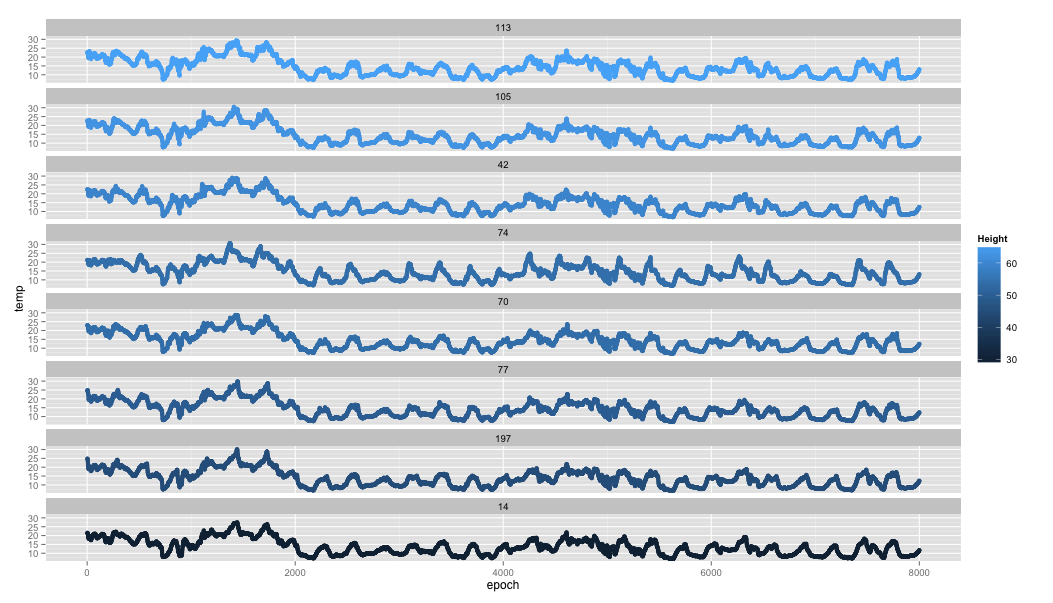
\includegraphics[width=\linewidth]{tempheightepoch}
\caption{Time-series for sampled 5 nodes: Temp versus Height}

\end{figure}

\begin{figure}[H]

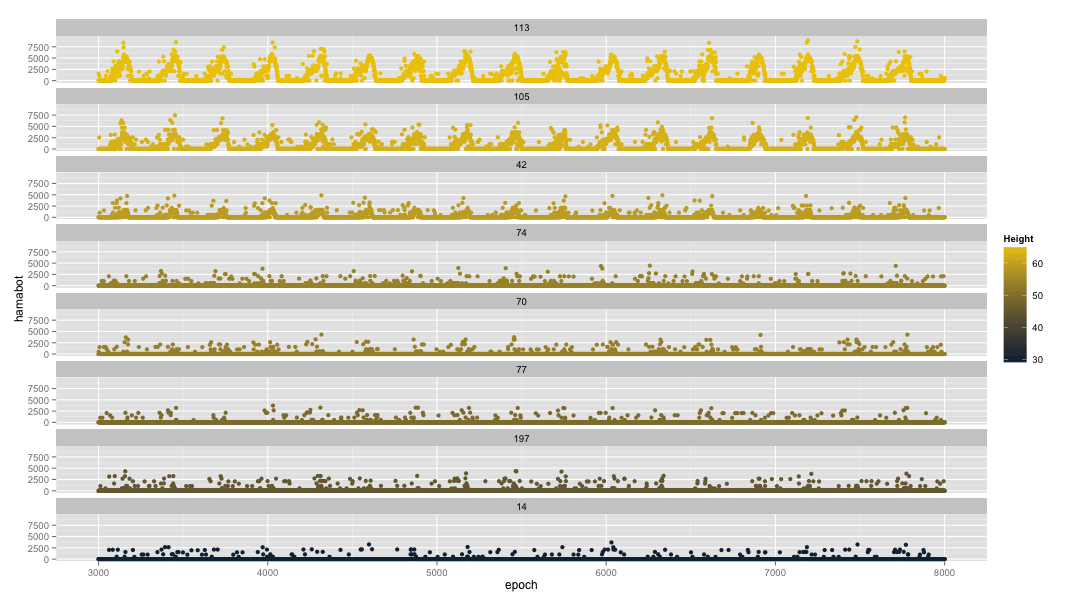
\includegraphics[width=\linewidth]{samplehama}
\caption{Timeseries for sampled 5 nodes: Hamabot versus Height}

\end{figure}


\subsection{Second finding}

\begin{figure}[H]

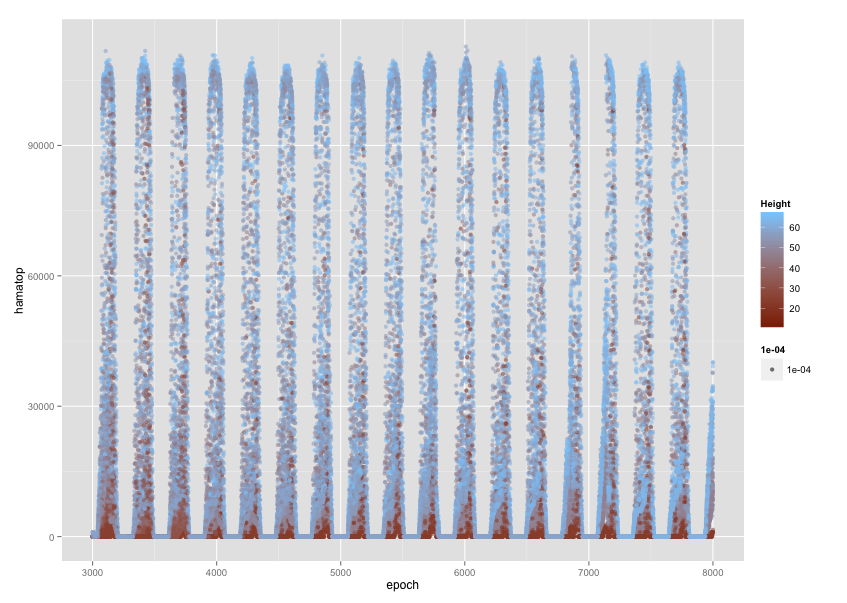
\includegraphics[width=\linewidth,height=350pt]{hamatime}
\caption{Timeseries for hamatop distribution coloured by Height}


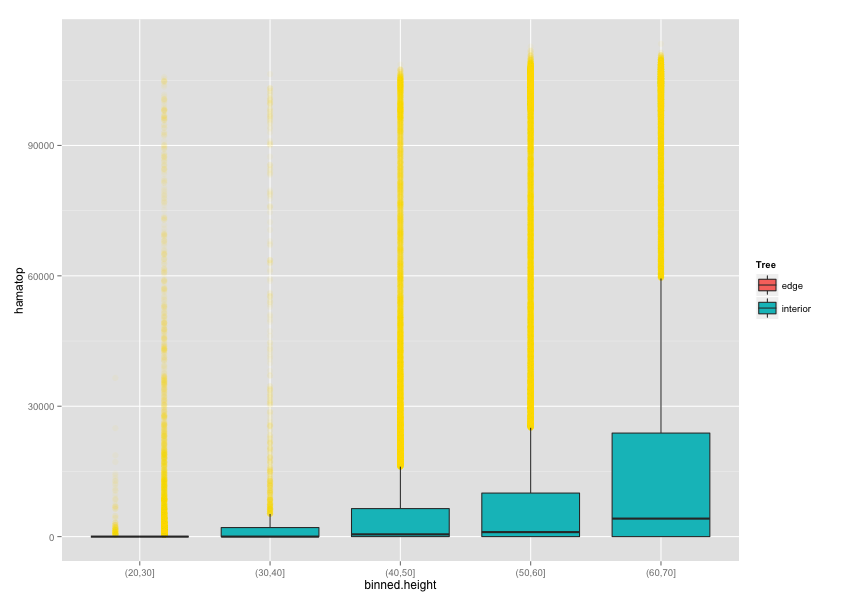
\includegraphics[width=\linewidth,height=350pt]{boxplothama}
\caption{Box-plot of hamatop distribution binned by Height of node}

\end{figure}

My second finding plots the same dataset in two graphical forms.  They study the relationship of direct PAR readings with time, and colours by height.  Again, we restrict the epoch duration to 3000-8000 to ensure a constant distribution of heights of the motes, to avoid this as a confounding factor.  The colour choice for height was meant to highly associations for higher heights with blue (canopy, skies) and lower with the earth.  The transparency helps us see that lower regions of the tree still had access to high direct PAR (so light from the sky), but in far fewer number.  The second plot, helps bring out this information in the form of box-plots, showing us that the outliers experiencing high direct PAR near the bottom of the tree were very sparse in comparison to those from the top.  Colouring by the tree (interior, exterior) brings to our attention that in this epoch interval, there were very few readings from the edge tree.  Which actually lessens an extra confounding factor (maybe the trees had very different foliage regions). 


\subsection{Third finding}
In the final finding, I present a scatterplot exploring the relationship between temperature and humidity.  I referred to this graph in the data exploration section, as the culmination of my investigating an aspect of the question of whether there are microclimates generated by the foliage of the tree.  The idea was that perhaps densely foliaged areas, which I assumed as tightly correlated with height, changed the relationship between humidity and temperature.  Sampling from the set of motes with more than 7000 observations, we make a faceted plot of temperature versus humidity, and discover that the correlation between the two has no relation to height.  
\begin{figure}[H]
\centering
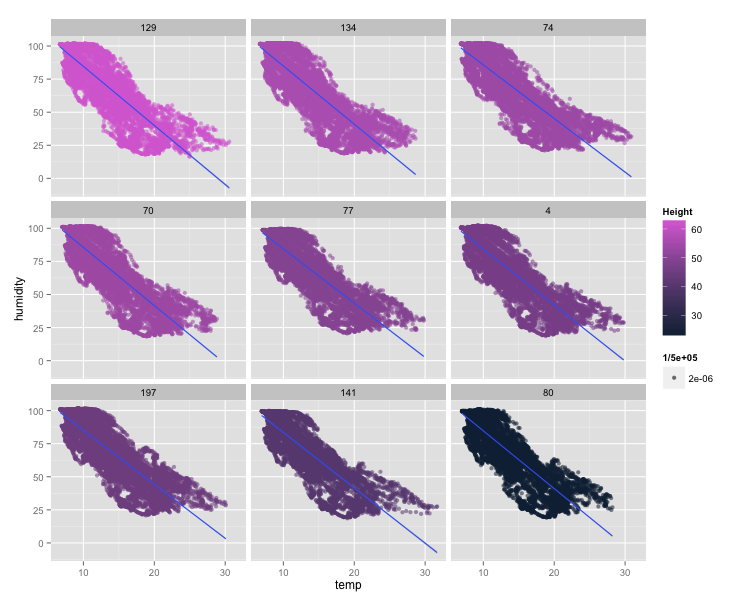
\includegraphics[width=\textwidth]{humidtemp7000}
\caption{Humidity versus Temperature: sampled 9 motes}

\end{figure}


\section{Discussion}

In approaching large datasets in the future, I would like to spend more time organizing different hypothesis so I can more exhaustively explore the data.  The dataset was large, so this was hard to do given the time/page-limit constraint, and I fear when I just do exploratory analysis that I am not being comprehensive enough, missing confounding factors.  I would've liked to create 3-D plots and animations given more time.   

\section{Conclusion}

The large data size did not feel restrictive, only perhaps what I can say about it in this lab. My findings and the plots in the exploration gave good indications of the relationships of the variables, however I do not feel enough analysis was made to conclude anything causal.  For instance, despite my third finding, it could still be the case that different foliage regions successfully buffers against the greater environment in another way.  I do not feel like I have exhausted what the dataset covers just yet.  

\end{document}
